\documentclass[12pt]{amsart}
\usepackage{amsmath,amsthm,amssymb,amsfonts,enumerate,mymath,tikz-cd,fancyhdr,multicol,graphicx}
\openup 5pt
\author{Blake Farman\\University of South Carolina}
\title{Math 116\\Exam 01}
\date{October 31, 2016}
\pdfpagewidth 8.5in
\pdfpageheight 11in
\usepackage[margin=1in]{geometry}

\renewcommand{\qedsymbol}{}
\theoremstyle{definition}
\newtheorem{thm}{}
\newtheorem{lem}{Lemma}
\theoremstyle{definition}
\newtheorem{defn}{Definition}
\newtheorem{rmk}{Remark}
\begin{document}
\maketitle

\begin{center}
  \fbox{\fbox{\parbox{5.5in}{\centering
        Answer the questions in the spaces provided on the
        question sheets and turn them in at the end of the class period.
        If you require extra space, use the back of the page and indicate that you have done so.
        
        Unless otherwise stated, all supporting work is required.
        Unsupported or otherwise mysterious answers will {\bf not receive credit.}
        You may {\it not} use any calculators.}}}
\end{center}

\vspace{0.2in}
\makebox[\textwidth]{Solutions}
\vspace{0.2in}

$$
\begin{array}{|c|c|c|}
  \hline
  \text{Problem} & \text{Points Earned} & \text{Points Possible}\\
  \hline
  1 & & 6\\
  \hline
  2 & & 1\\
  \hline
  3 & & 1\\
  \hline
  4 & & 2\\
  \hline
  5 & & 18 \\
  \hline
  6 & & 18\\
  \hline
  7 & & 18\\
  \hline
  8 & & 18\\
  \hline
  9 & & 18\\
  \hline
  \text{Total} & & 100\\
  \hline
\end{array}
$$

\newpage

\section{Definitions}

\begin{thm}[6 Points]\label{ex2}
  Let $a, b$ be non-zero real numbers and $m, n$ rational numbers.
  Fill in the blanks
  \begin{multicols}{2}
    \begin{enumerate}[(i)]
    \item
      $\displaystyle{a^0 = 1}$,
      \vspace{.15in}
    \item
      $\displaystyle{\left(\frac{a}{b}\right)^{-n} = \frac{b^n}{a^n}}.$
      \vspace{.15in}
    \item
      $\displaystyle{a^m \cdot a^n = a^{m+n}}$
      \vspace{.15in}
    \item
      $\displaystyle{\frac{a^m}{a^n} = a^{m-n}}$
      \vspace{.15in}
    \item
      $\displaystyle{\left(a \cdot b\right)^n = a^n\cdot b^n}$
      \vspace{.15in}
    \item
      $\displaystyle{\left(\frac{a}{b}\right)^n = \frac{a^n}{b^n}}$
    \end{enumerate}
  \end{multicols}
\end{thm}

\begin{thm}[1 Points]\label{ex3}
  State the Quadratic Formula.
  That is, state the solutions of the equation $ax^2 + bx + c = 0$.
  $$x = \frac{-b \pm \sqrt{b^2 - 4ac}}{2a}$$
\end{thm}

\begin{thm}[1 Points]\label{ex4}
  Fill in the blanks:\\
  \begin{center}
    To make $x^2 + bx$ a perfect square, add and subtract $\left(\frac{b}{2}\right)^2$\,.
    This gives
    $$x^2 + bx + \left(\frac{b}{2}\right)^2 - \left(\frac{b}{2}\right)^2 = \left(x + \frac{b}{2}\right)^2 - \left(\frac{b}{2}\right)^2.$$
  \end{center}
\end{thm}

\begin{thm}[2 Points]\label{ex1}
  \begin{enumerate}[(a)]
  \item
    State the Point-Slope form of a line passing through the point $(x_0, y_0)$ with slope $m$.
    $$y - y_0 = m(x - x_0)$$
  \item
    State the Slope-Intercept form of a line with slope $m$ and $y$-intercept $b$.
    $$y = mx + b$$
  \end{enumerate}
\end{thm}
\newpage
\section{Exercises}

\begin{thm}[18 Points]\label{ex5}
  In the following problems, use the given information to find the equation of the line in Slope-Intercept Form and then graph the lines.
  \begin{enumerate}[(a)]
  \item
    The line passing through the point $\left(\frac{1}{2}, 3\right)$ and parallel to the line $4y + 8x = 12$.
    \begin{proof}[Solution]
      First we determine the slope of $4y + 8x = 12$ by putting the equation into slope-intercept form.
      Subtract $8x$ from both sides of the equation to get $4y = -8x + 12$, then divide both sides by $4$ to get
      $$y = \frac{-8x + 12}{4} = \frac{4(-2x + 3)}{4} = -2x + 3.$$
      Any line parallel to the given line has the same slope, so the equation of the parallel line passing through $\left(\frac{1}{2},3\right)$ in point-slope form is 
      $$y - 3 = -2\left(x - \frac{1}{2}\right).$$
      To put this into slope-intercept form, add 3 to both sides and expand to get
      $$y = -2\left(x - \frac{1}{2}\right) + 3 = -2x + 2\cdot\frac{1}{2} + 3 = -2x + 1 + 3 = -2x + 4.$$
      The graphs of these lines are then
      \begin{center}
        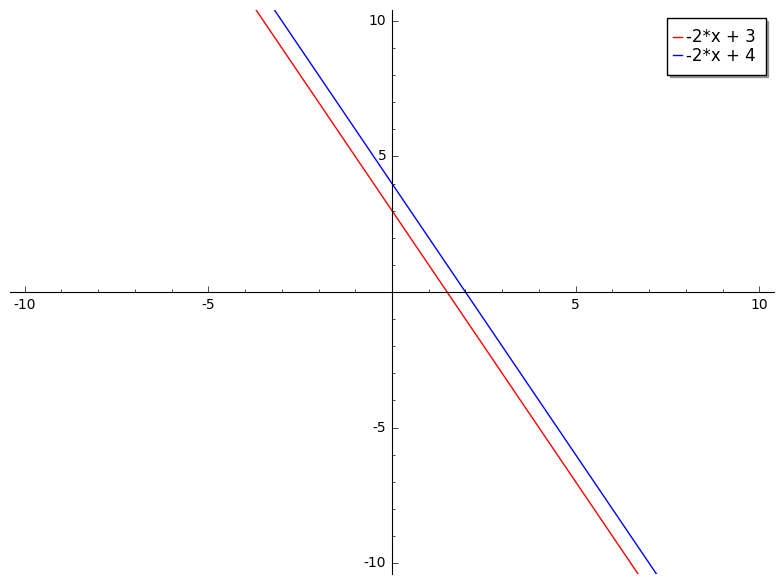
\includegraphics[scale=0.5]{imgs/ParallelLines.png}
      \end{center}
    \end{proof}
    \newpage
  \item
    The line passing through the  point $\left(\frac{1}{3},5\right)$ and perpendicular to the line $3y - x = 9$.
    \begin{proof}[Solution]
      First we put the given line into slope-intercept form so we can read off the slope.
      We add $x$ to both sides to get
      $$3y = x + 9$$
      then divide both sides by 3 to get
      $$y = \frac{x + 9}{3} = \frac{x}{3} + \frac{9}{3} = \frac{1}{3}x + 3,$$
      hence the slope is $\frac{1}{3}$.
      The slope, $m$, of a line perpendicular to the given line satisfies
      $$m\cdot \frac{1}{3} = -1$$
      and so multiplying both sides by $3$ we find $m = -1 \cdot 3 = -3$.
      The line perpendicular to the given line passing through $\left(\frac{1}{3},5\right)$ in point-slope form is then
      $$y - 5 = -3\left(x - \frac{1}{3}\right).$$
      To put this into slope-intercept form, we add 5 to both sides and expand to get
      $$y = -3\left(x - \frac{1}{3}\right) + 5 = -3x + 3 \cdot \frac{1}{3} + 5= -3x + 1 + 5 = -3x + 6.$$
      The graphs of these lines are then
      \begin{center}
        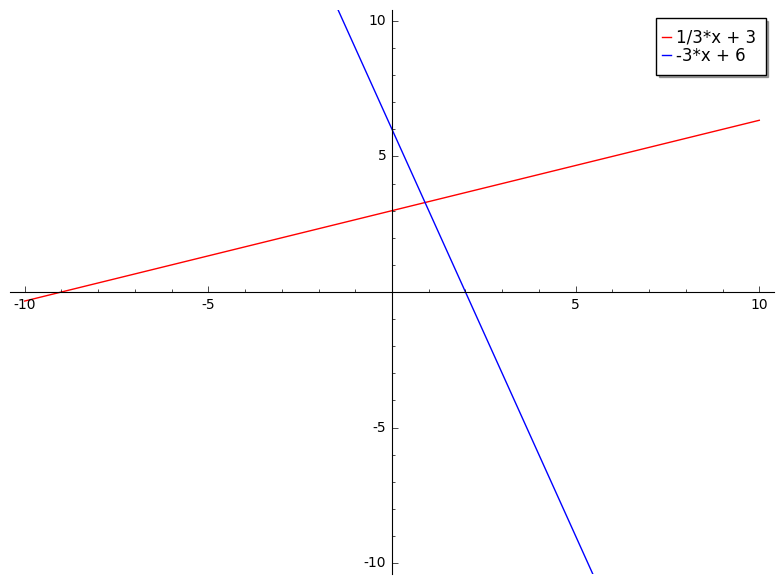
\includegraphics[scale=0.5]{imgs/PerpendicularLines.png}
      \end{center}
    \end{proof}
  \end{enumerate}
\end{thm}

\newpage
\begin{thm}[18 Points]\label{ex9}
  Find all solutions, real and complex, to the equation
  $$x^2 + x + 1 = 0.$$
  \begin{proof}[Solution]
    Using the quadratic formula we get
    \begin{eqnarray*}
      x &=& \frac{-1 \pm \sqrt{1^2 - 4(1)(1)}}{2(1)}\\
      &=& \frac{-1 \pm \sqrt{1 - 4}}{2}\\
      &=& \frac{-1 \pm \sqrt{-3}}{2}\\
      &=& \frac{-1 \pm \sqrt{-1}\sqrt{3}}{2}\\
      &=& \frac{-1 \pm i\sqrt{3}}{2}.
    \end{eqnarray*}
  \end{proof}
\end{thm}

\begin{thm}[18 Points]\label{ex10}
  \begin{enumerate}[(a)]
  \item
    Complete the square for the function $f(x) = x^2 - x - 6$.
    \begin{proof}[Solution]
      To complete the square we add and subtract $\left(\frac{1}{2}\right)^2$ to get
      \begin{eqnarray*}
        f(x) &=& x^2 - x - 6\\
        &=& x^2 - x + \left(\frac{1}{2}\right)^2 - \left(\frac{1}{2}\right)^2 - 6\\
        &=& \left(x - \frac{1}{2}\right)^2 - \frac{1}{4} - \frac{24}{4}\\
        &=& \left(x - \frac{1}{2}\right)^2 - \frac{25}{4}.
      \end{eqnarray*}
    \end{proof}
  \item
    Solve $f(x) = 0$.
    \begin{proof}[Solution]
      Since we've already completed the square, we can just solve
      $$f(x) = \left(x - \frac{1}{2}\right)^2 - \frac{25}{4} = 0.$$
      First add $\frac{25}{4}$ to both sides to get
      $$\left(x - \frac{1}{2}\right)^2 = \frac{25}{4},$$
      then take the the square root of both sides to get
      $$x - \frac{1}{2} = \pm \sqrt{\frac{25}{4}} = \pm \frac{\sqrt{25}}{\sqrt{4}} = \pm \frac{5}{2}$$
      and finally add $\frac{1}{2}$ to both sides to get
      $$x = \frac{1}{2} \pm \frac{5}{2} = \frac{1 \pm 5}{2}.$$
      Therefore the solutions are
      $$x = \frac{1 + 5}{2} = \frac{6}{2} = 3\ \text{or}\ x = \frac{1 - 5}{2} = \frac{-4}{2} = -2.$$
      \begin{rmk}
        This is exactly what we would get if we applied the quadratic formula; indeed, completing the square and then solving for the roots is just rederiving the quadratic formula for this specific polynomial.
        Additionally, we could have also factored
        $$f(x) = x^2 - x - 6 = (x - 3)(x + 2)$$
        and observed that the solutions to 
        $$f(x) = (x - 3)(x + 2) = 0$$
        are thus $x = 3$ or $x = -2$.
      \end{rmk}
    \end{proof}
  \item
    Use the information from parts (a) and (b) to sketch a graph of $f(x)$.
    Label the $y$-intercept, any $x$-intercept(s), and the vertex.
    \begin{proof}[Solution]
      The $y$-intercept is the point $(0, f(0)) = (0,-6)$.
      We can read the vertex from the completed square:
      $$f(x) = \left(x - \frac{1}{2}\right)^2 - \frac{25}{4}$$
      tells us that the vertex is $\left(\frac{1}{2},-\frac{25}{4}\right)$.
      Part~(b) of this problem gives us the two $x$-intercepts, $(-2,0)$ and $(3,0)$.
      Therefore the graph of $f(x)$ is 
      \begin{center}
        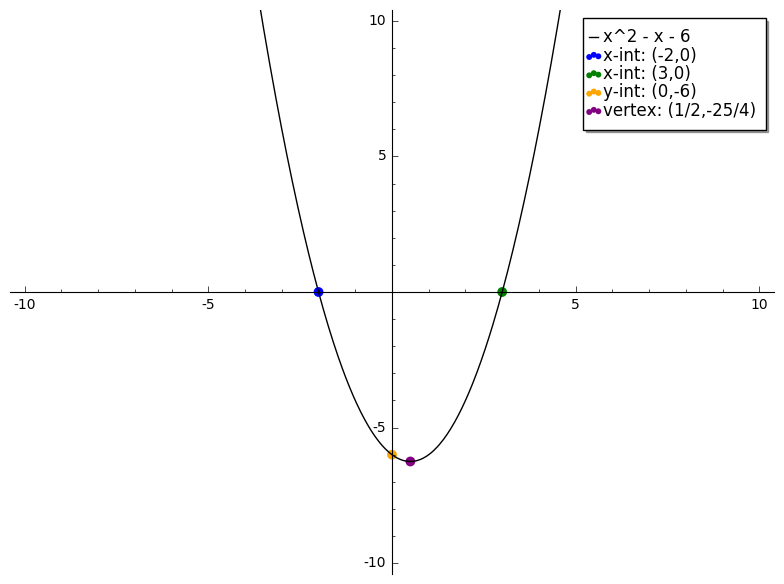
\includegraphics[scale=0.5]{imgs/Parabola.png}
      \end{center}
    \end{proof}
  \end{enumerate}
\end{thm}

\begin{thm}[18 Points]\label{ex9}
  Find all solutions, both real and complex, of the equation
  $$x + \sqrt{x} + 1 = 0.$$
  \begin{proof}[Solution]
    The easiest way to solve this problem is to subtract $\sqrt{x}$ from both sides to get
    $$-\sqrt{x} = x + 1$$
    then square both sides to get
    $$x = (x + 1)^2 = x^2 + 2x + 1$$
    and finally subtract $x$ from both sides to obtain the equation
    $$0 = x^2 + 2x + 1 - x = x^2 + x + 1,$$
    which we have already solved in Problem~6.
    Therefore the solutions are
    $$x = \frac{-1 \pm i\sqrt{3}}{2}.$$
    
    If the reduction is not obvious, one can always solve this problem by making the substitution $y = \sqrt{x}$ so that
    $$y^2 + y + 1 = (\sqrt{x})^2 + (\sqrt{x}) + 1 = x + \sqrt{x} + 1 = 0$$
    and then apply the quadratic formula to get
    $$y = \frac{-1 \pm \sqrt{1^2 - 4(1)(1)}}{2(1)} = \frac{-1 \pm \sqrt{-3}}{2} = \frac{-1 \pm i\sqrt{3}}{2}.$$
    Finally, we recall that $y = \sqrt{x}$ and we want the values of $x$, so we have the two solutions
    \begin{eqnarray*}
      x &=& y^2\\
      &=& \left(\frac{-1 + i\sqrt{3}}{2}\right)^2\\
      &=& \frac{\left(-1 + i\sqrt{3}\right)^2}{2^2}\\
      &=& \frac{(-1)^2 + 2(-1)(i\sqrt{3}) + (i\sqrt{3})^2}{4}\\
      &=& \frac{1 - 2i\sqrt{3} + i^2\sqrt{3}^2}{4}\\
      &=& \frac{1 - 2i\sqrt{3} + (-1)(3)}{4}\\
      &=& \frac{1 - 3 - 2i\sqrt{3}}{4}\\
      &=& \frac{-2 - 2i\sqrt{3}}{4}\\
      &=& \frac{2(-1 - i\sqrt{3})}{4}\\
      &=& \frac{-1 - i\sqrt{3}}{2}
    \end{eqnarray*}
    or, similarly,
    \begin{eqnarray*}
      x &=& y^2\\
      &=& \left(\frac{-1 - i\sqrt{3}}{2}\right)^2\\
      &=& \frac{-1 + 2i\sqrt{3} - 3}{4}\\
      &=& \frac{-2 + 2i\sqrt{3}}{4}\\
      &=& \frac{-1 + i\sqrt{3}}{2}.
    \end{eqnarray*}
  \end{proof}
\end{thm}

\begin{thm}[18 Points]\label{ex9}
  Find the simultaneous solutions to the following system
  $$\left\{\begin{array}{rcl}
    y &=& x^2 + 2x + 3,\\
    y &=& x + 5.
  \end{array}\right.$$

  \begin{proof}[Solution]
    To find the $x$-values of the simultaneous solutions we solve
    $$x + 5 = x^2 + 2x + 3$$
    for $x$.
    Subtracting $x + 5$ from both sides gives 
    $$0 = x^2 + 2x + 3 - (x + 5) = x^2 + 2x + 3 - x - 5 = x^2 + x - 2 = (x + 2)(x - 1).$$
    Hence $x = -2$ or $x = 1$.
    The corresponding $y$-values are $y = (-2) + 5 = 3$ and $y = (1) + 5 = 6$.
    Therefore the simultaneous solutions are
    $$(-2, 3)\ \text{and}\ (1,6).$$
    
    Graphically, these are just the two points of intersection of the line $y = x + 5$ and the parabola $y = x^2 + 2x + 3$:
    \begin{center}
      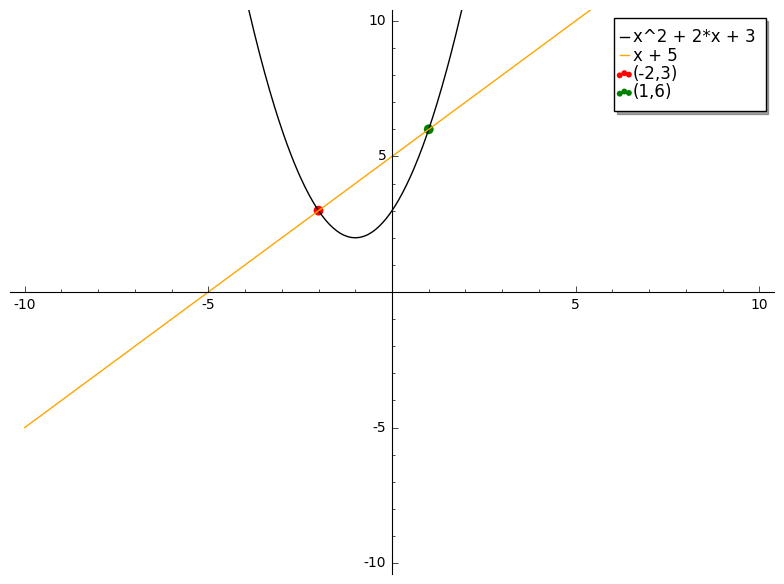
\includegraphics[scale=0.5]{imgs/Intersection.png}
    \end{center}
  \end{proof}
\end{thm}
\end{document}
